\documentclass{article}
\usepackage[utf8]{inputenc}
\usepackage{graphicx}
\usepackage{amsthm}
\usepackage{amssymb}
\usepackage{amsfonts}
\usepackage{color}
\usepackage{enumitem}
\title{Projet: \\ Chiffre de César et Chiffre de Vigenère}
\author{SABABADY Kamala et SELVARAJAH Dinusan}
\begin{document}
\maketitle
\section{{\color{red}Partie 1 :}  \textit{Le chiffre déchiffrable de Jules César}}
$$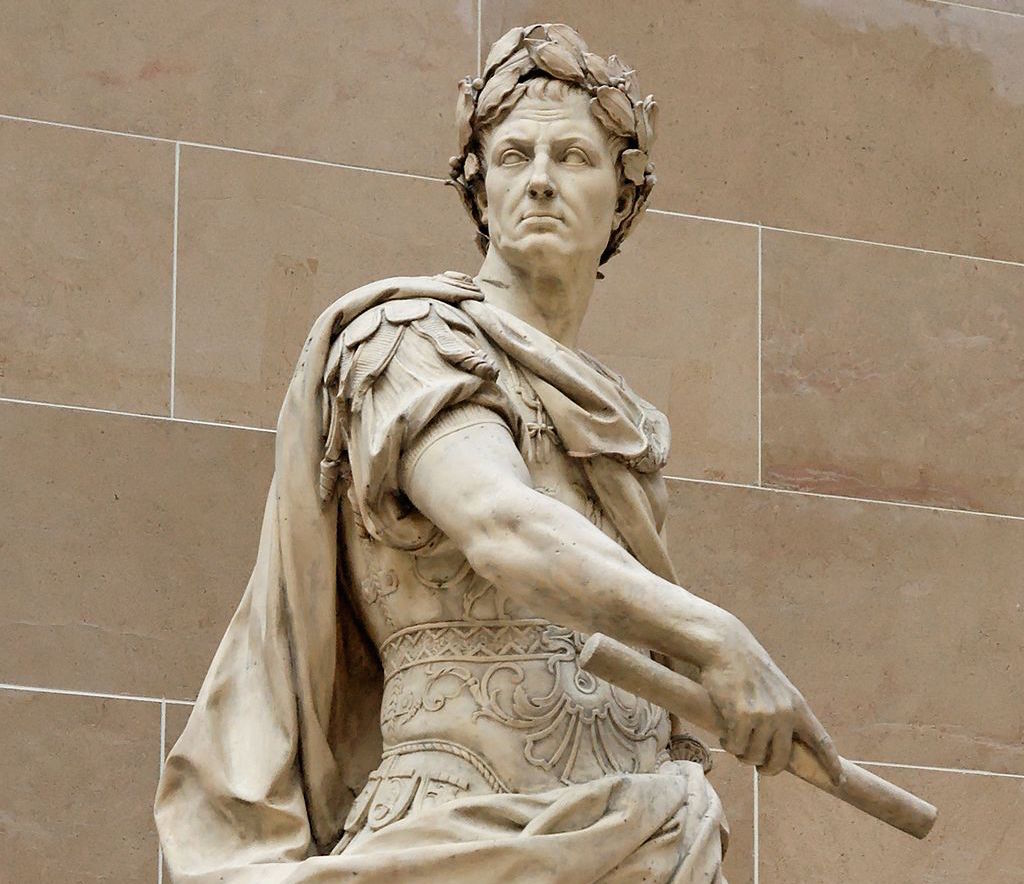
\includegraphics[width=5cm]{c.jpg}$$
 \textit{Jules Cesar (100 av.J.-C - 44 av.J.-C), celebre empereur romain}
\\

Jules César , célèbre empereur romain a utilisé la cryptographie en inventant le chiffrement par décalage c'est à dire il rendait illisibles ses messages pour se protéger de ses ennemis au cas où ses messages tombent entre leurs mains. Vous allez voir que sa technique était très simple à comprendre mais aussi à pirater . 
\\

Par exemple imaginons que Jules veut envoyer ce message "  allez les bleus " , il aimait utiliser le chiffre 3 comme clé pour procéder à son cryptage mais nous on peut changer ce chiffre donc voyons ce que ça donne avec le chiffre 2 :
\\

La première lettre du message est "  ". Il s’agit de la première lettre de l’alphabet. $1 + 2 = 3$. " C " est la troisième lettre de l’alphabet. " A " est donc remplacé par " C ".
\\

La deuxième lettre du message est " L ". Il s’agit de la douzième lettre de l’alphabet. $12 + 2 = 14.$ " N " est la quatorzième lettre de l’alphabet. " L " est donc remplacé par " N ". 
Et ainsi de suite... 
Le message crypté donne à la fin "CNNGABNGUBDNGWU".
\\

Nous avons crée un programme qui code un message par la méthode de César, qui dès le début demande à l'utilisateur le message à crypter et la clé , qui renvoie un message crypté. 
\\

On a commencé à créer une variable "lettres" avec les 26 lettres de l'alphabet puis on a créé une variable "crypted" qui reçoit notre message crypté. 
Pour chercher chaque caractère du message on a définit une boucle \textit{for}.
\\

Pour décrypter les messages, le code est essentiellement le même, sauf qu’on remplace le message original par le message crypté. Aussi, on soustraie la clé au lieu de l’additionner.
\\

 Voici quelques exemples:
\begin{itemize}[label=\textbullet, font=\LARGE \color{black}]
\item \textbf{Message:} \textit{licence maths}
\item \textbf{Clé:} \textit{3}
\item \textbf{Message crypté:}  \textit{olfhqfh pdwkv}
\end{itemize}
$$ $$
\begin{itemize}[label=\textbullet, font=\LARGE \color{black}]
\item \textbf{Message:} \textit{python}
\item \textbf{Clé:} \textit{9}
\item \textbf{Message crypté:}  \textit{yhcqxw}
\end{itemize}
Jules César se disait que personne ne pourrait déchiffrer ses messages mais le problème c'est que sa méthode est simpliste et dans un alphabet de 26 lettres, Jules César n’avait que 26 choix de décalage c'est peu pour crypter donc il est facilement décryptable.
\\
\section{{\color{red}Partie 2 :}  \textit{Le chiffre indéchiffrable de Blaise de Vigenère}}
$$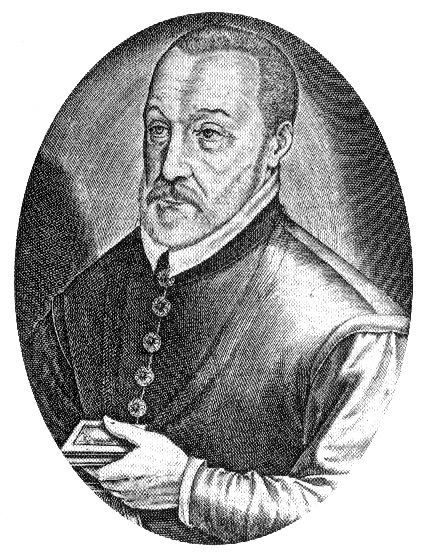
\includegraphics[width=5cm]{v.jpg}$$
\textit{Blaise de Vigenere (1523-1596), diplomate francais.}
\\

À la fin du Moyen-Âge, en France, \textit{le diplomate français Blaise de Vigenère} (qui avait de toute évidence un intérêt pour les mathématiques) met au point un algorithme que personne ne réussira à briser pendant plus de \textbf{250 ans!}\\

De Vigenère a présenté sa méthode devant la cour d’Henri III en 1586. L’algorithme se révèle particulièrement coriace pour les scientifiques et savants de l’époque qui tentent de le déchiffrer, ce qui lui vaudra le surnom de \textit{\textbf{chiffre indéchiffrable}}.\\

La méthode de Vigenère consistait à choisir une clé et à s’en servir pour crypter le message lui-même. Par exemple, imaginons la situation suivante:
\begin{itemize}[label=\textbullet, font=\LARGE \color{black}]
\item \textbf{Message:} \textit{Le chiffre indéchiffrable}
\item \textbf{Clé:} \textit{python}
\end{itemize}
$$ $$
Voici comment nous nous y prendrions pour crypter notre message dans Excel. Les deux premières lignes représentent notre alphabet avec le chiffre correspondant à chaque lettre (en Python, on commence toujours nos listes par 0).\\

Nous avons ensuite la ligne de notre message, avec le numéro de chaque lettre, puis notre clé, qui se répète pour couvrir tout le message, et avec encore une fois le chiffre correspondant à chaque lettre.\\

Pour crypter notre message, il suffit de faire la somme des chiffres correspondant à la lettre en clair et à la lettre de notre clé. Par exemple, la première lettre du message est " L ", qui est associé à 11. La lettre correspondante pour notre clé est " P ", qui est le numéro " 15 ". $11 + 15 = 26$. Nous n’avons pas de lettre 26, donc nous retournons au début, ce qui nous donne la lettre " A "!\\


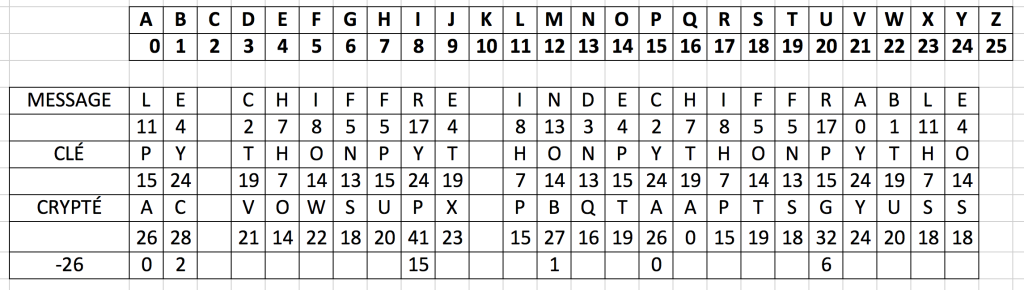
\includegraphics[width=15cm]{t.png}\\

La grande force de cette technique réside dans le fait qu’une lettre peut servir à en crypter plusieurs autres. Par exemple, le " Y " de notre clé " PYTHON " sert à crypter " E ", " R ", " C " et " A ". À l’inverse, les lettres cryptées peuvent aussi renvoyer à plusieurs lettres en clair. Dans le message crypté, " A " renvoie tant " L " qu’à " C " et " H ".\\

De plus, avec six lettres, il existe $26^6 = 308 915 776$ clés possibles! Et si on avait fait un petit effort supplémentaire avec une clé de 10 lettres, on aurait eu le choix entre $141 167 095 653 376$ combinaisons différentes!  Pas étonnant que les mathématiciens se soient cassés les dents pendant près de trois siècles sur cet algorithme. Il y a beaucoup trop de possibilités pour toutes les tester, même avec un ordinateur!\\

Nous avons crée un programme qui code un message par la méthode de Vigenère, qui dès le début demande à l'utilisateur le message à crypter et la clé , qui renvoie un message crypté. 
\\

Nous avons testé notre programme avec quelques exemples:
\begin{itemize}[label=\textbullet, font=\LARGE \color{black}]
\item \textbf{Message:} \textit{Bonjour}
\item \textbf{Clé:} \textit{hello}
\item \textbf{Message crypté:}  \textit{ISYUCBV}
\end{itemize}
$$ $$

\begin{itemize}[label=\textbullet, font=\LARGE \color{black}]
\item \textbf{Message:} \textit{no pain no gain}
\item \textbf{Clé:} \textit{motivate}
\item \textbf{Message crypté:}  \textit{ZC IIDN GS SOBV}
\end{itemize}
$$ $$ 

\begin{itemize}[label=\textbullet, font=\LARGE \color{black}]
\item \textbf{Message:} \textit{sans effort il n'y a pas de résultat}
\item \textbf{Clé:} \textit{qui ne tente rien n'a rien}
\item \textbf{Message crypté:}  \textit{IUVR RJEHVG BP M'P I TNR QD RÉRLTXNJ}
\end{itemize}
$$ $$

Enfin pour décrypté il sufffit de inverser le processus. Nous avons également crée un programme qui décrypte un message. 


\end{document}

